\documentclass{article}
\usepackage[utf8]{inputenc}
\usepackage{amsmath}
\usepackage{graphicx}
\graphicspath{ {./images/} }

\title{Tarea 03 de Circuitos Lineales I}
\author{Gabriel Gamboa Vargas}
\date{Octubre 2021}

\begin{document}

\maketitle
\section{Ejercicio 1}
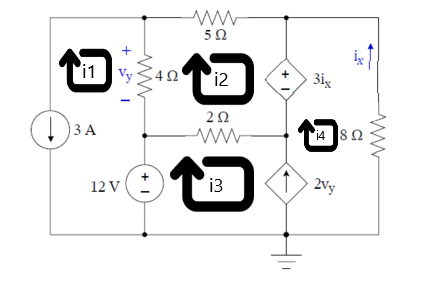
\includegraphics[]{images/ejercicio1.PNG}

\begin{equation} 
    i1 = -3A
\end{equation}
 
\begin{equation} 
    i4 = -ix
\end{equation}

\begin{equation} 
   {4\Omega} i1 - {4\Omega} i2 + {2\Omega}i3 - {2\Omega}i2 +3i4 - {5\Omega}i2 = 0
\end{equation}
\\ \\
 Se usa un supernodo desde i3 hasta i4, donde hay una fuente de corriente.\\

\begin{equation}
   -12V + {2\Omega}i3 -{2\Omega}i2 + 3i4 + {8\Omega}i4 = 0
\end{equation}
Con una limitación dada por la fuente de corriente de valor 2Vy: \\

\begin{equation}
   i4 - i3 = {8\Omega}i1 -{8\Omega}i2
\end{equation}
\\ En forma matricial: \\ \\ 

$
\begin{pmatrix}
    1 & 0 & 0 & 0 \\
    4 & -11 & 2 & 3 \\
    0 & -2 & 2 & 11\\
    -8 & 8 & -1 & 1
\end{pmatrix}
$$\begin{bmatrix}
    i1 \\
    i2 \\
    i3 \\
    i4 
\end{bmatrix}
$ = $\begin{bmatrix}
    -3 \\
    0 \\
    12  \\
    0
\end{bmatrix}
$ \\ \\ \\
$i1 = -3A$ \\ \\
$i2 = 57.6A$ \\ \\
$i3 = 420A$ \\ \\
$i4 = -64.8A$\\
\section{Ejercicio 2}

\begin{equation}
    i1 - i3 = Bib
\end{equation}

\begin{equation}
    i2 - i3 = ib
\end{equation}
Se aplica (6) / (7)\\ 
\begin{equation}
    B = \frac{i1-i3}{i2 -i3} = \frac{37}{6}
\end{equation}
Note: \\
$Va={20\Omega}(i2 - i1) = 77.5V$ \\ 
${50\Omega}(i2 - i3) = -37.5V$\\ 
${20\Omega}i3 = 65V$\\  \\
Se aplica LTK para obtener:\\ \\
$ -10V - 65V + A77.5V -37.5V+ 77.5V = 0$
\begin{equation}
    A = \frac{-77.5V + 37.5V +65V + 10V}{77.5V} = \frac{14}{31}
\end{equation}
\section{Ejercicio 3}
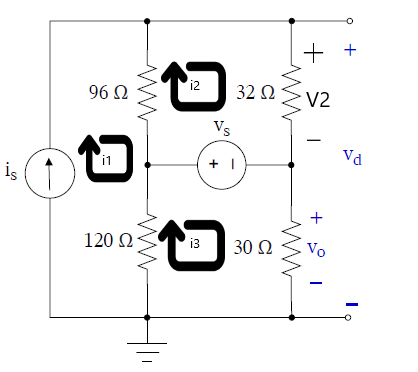
\includegraphics[]{images/ejercicio2.PNG} \\
Note: \\ 
$is = i1$ \\
${96\Omega}is - {96\Omega}i2 + Vs - {32\Omega}i2 = 0$  \\
${120\Omega}is - {120\Omega}i3 - Vo - Vs = 0$ \\
$4Vo = {120\Omega}i3$ \\ \\ 
Simplificando: \\

\begin{equation} 
    {96\Omega}is - {128\Omega}i2 + Vs = 0
\end{equation}

\begin{equation}
    {120\Omega}is - 5Vo - Vs = 0
\end{equation}
Se aplica el teorema de superposición sobre la variable V2 que se muestra en la figura al inicio del ejercicio. Se usa la variable V1x para denotar el voltaje cuando se elimina la fuente de voltaje y V2x el voltaje cuando se elimina la fuente de corriente.\\  \\
Al remover la fuente de voltaje Vs el voltaje sobre los resistores de ${96\Omega}$ y ${32\Omega}$  es V1x, luego se aplica LCK para encontrar:\\
$is =\frac{V1x}{{96\Omega}} + \frac{V1x}{{32\Omega}} \Rightarrow   V1x = 24is$\\ \\
Al remover la fuente de corriente las resistencias de ${96\Omega}$ y ${32\Omega}$ quedan en serie, por lo tanto se cumple: \\ \\
$V2x = \frac{32Vs}{128} $\\ \\
Por el teorema de superposición: \\ \\
$V2 = V1x + V2x = 24is + \frac{32Vs}{128}$ \\ \\
Por lo tanto: \\ 
\begin{equation}
    i2 = \frac{3is}{4} + \frac{Vs}{128}
\end{equation}
Se aplica (10) -  (11) y se sustituye i2 de acuerdo con (12) \\ \\
$    {-24\Omega}is -Vs - 96is + 5Vo + 2Vs = 0$ \\
Al Simplificar:\\
\begin{equation}
    -120is  +Vs = -5Vo \Rightarrow  Vo = \frac{-Vs}{5} +24is
\end{equation}
\section{Ejercicio 4}
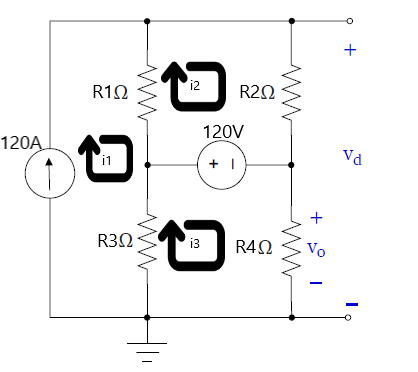
\includegraphics[]{images/ejercicio3.PNG} \\
$i1 = 120A$\\
De acuerdo con teorema de superposición aplicado para esta misma topología, se encontró:\\
$V2 = 120A(\frac{R1*R2}{R1+R2}) + 120V(\frac{R2}{R1+R2})$ \\ \\
$i2 =   120A(\frac{R1}{R1+R2}) + 120V(\frac{1}{R1+R2})$\\  \\
\begin{equation}
    i2 = 120(\frac{R1 + 1}{R1 + R2})
\end{equation}
Se aplica LTK para encontrar una expresión i3\\ \\
$R3i3 -R3*120A + 120V +R4i3 =0$\\ \\
$ i3= \frac{-120V+R3*120A}{R4+R3}$ \\ \\
\begin{equation}
    i3 = 120(\frac{R3 -1}{R3 + R4})
\end{equation}
Note que por LTK: \\ \\
$Vd = R4*i3 + R2*i2$ \\ \\
$Vd = 120R4(\frac{R3 - 1}{R3 + R4}) + 120R2(\frac{R1 + 1}{R1 + R2})$ \\ \\
Note que si se le asignan valores de ${1\Omega}$ a todas las resistencias Vd = 120V y a medida que las resistencias crecen Vd crece también, así que el diseño debe de ser poco convencional. \\ \\
Para resolver esto se cambian las resistencias R1 y R2 por cortos de la siguiente forma\\ \\ 
\includegraphics[]{images/ejercicio4diseño.PNG} \\
Para conseguir una resistencia de ${1\Omega}$ vamos a utilizar resistencias comerciales de ${10\Omega}$ con el siguiente código de colores. \\ \\
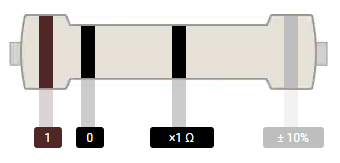
\includegraphics[]{images/resistencia.PNG} \\
Se unen 10 resistencias de ${10\Omega}$ en paralelo y se consigue:\\ 
\begin{equation}
    R3 = (\frac{10}{{10\Omega}})^{-1} = {1\Omega}
\end{equation}
Utilizando resistencias de ${12\Omega}$ con el código de colores \\ \\
 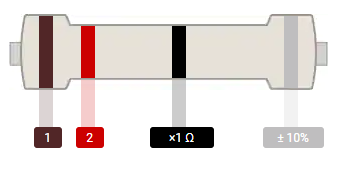
\includegraphics[]{images/resistencia1.PNG} \\
Se unen 15 resistencias comerciales en paralelo para obtener: \\ \\
\begin{equation}
    R4 = (\frac{15}{{12\Omega}})^{-1} = {0.8\Omega}
\end{equation}
La fórmula de Vd se indefine para este diseño poco convencional, pero se puede resolver utilizando el teorema de superposición y se encuentra: \\ \\
\begin{equation}
    Vd = 53.333V
\end{equation}
Este resultado se acerca mucho al deseado pero se necesita demasiadas resistencias en paralelo lo cual lo vuelve poco práctico. Siempre se puede adaptar para que sea menos exacto pero más sencillo de fabricar si fuera requerido.
\end{document}